\chapter*{Introduction}\label{chap:intro}\setcounter{page}{1}\frontmatter
\addcontentsline{toc}{chapter}{Introduction}
\chaptermark{Introduction}

When answering the classic question ``What is your Ph.D. about?'' to family and friends, I always start with the ``Ctrl + F'' function in their favourite text editor or web browser. This quickly highlights one of the applications of the exact pattern-matching problem. If I feel especially ambitious in my explanations, I will attempt to give the intuition of the naive $\Oh(nm)$ algorithm. Picture a young child, aligning the string against every position of the text and comparing character by character because the child has yet to learn how to read. To show a glimpse of a more complex solution, I comment on how, depending on the pattern, the child may try to skip portions of the text. But even my grandparents immediately know that efficient search in a text has been possible for decades and that it cannot be my real research subject.

\section{Context}

Indeed, exact pattern matching has been long studied, with in particular the famous Knuth-Morris-Pratt algorithm\footnote{The elegance of this algorithm is what first drew me in this area of research as a bachelor student!} published in 1977~\cite{KMP} after being independently discovered by Morris-Pratt in a technical report in 1970 and Knuth in 1973. Since then, this has become one of the classic textbook algorithms, and Charras and Lecroq published a detailed handbook~\cite{charras2004handbook} on the various solutions to exact pattern matching.

\subsection{Matching Models}\label{sec:intro:complex}

% Define center type column
\newcolumntype{Y}{>{\centering\arraybackslash}X}
\newcolumntype{P}[1]{>{\centering\arraybackslash}m{#1}}
\renewcommand\tabularxcolumn[1]{m{#1}}

%spacing
\renewcommand{\arraystretch}{2}
\begin{figure}[h]
    \begin{tabularx}{\textwidth}{P{3cm} P{4.5cm}  Y }
        Matching model & Pattern & Text with occurences underlined \\
        \hline
        Regular Expression~\cite{RM-704} & $P=$ GAT$(\mathrm{TA}\mid \mathrm{O})(\mathrm{CAT})^*$ & $T=$ \underline{GATTA}AT\underline{GATOCATCATCATCAT}A \\
        Error bound~\cite{landau1986efficient} (for ED~\cite{levenshtein1966binary}) & $P=$ GATTACAT & $T=$ AT\underline{GATTAACAT}ATA, $\mathrm{ED}(P,T[2..10])=1$ \\
        Don't care~\cite{fischer1974string} & $P=$ GAT**CAT & \underline{GATTACAT}A\underline{GATOACAT}AC\\
        %
        Gapped consecutive~\cite{bille2022gapped} & $P_1=$ GATTA $P_2=$ TAC  $a=2$, $b=6$ & $T=$ AGG\underline{GATTAC}TAC, $d=3 \in [a,b]$\\
        %
        Elastic Degenerate~\cite{iliopoulos2021efficient}  & $P=$ GATTACAT &  $T=$ {\renewcommand{\arraystretch}{1} AT\underline{GAT}$\left\{
            \begin{array}{l}
                \mathrm{\underline{TA}}  \\
                \mathrm{O}
            \end{array}\right\} \mathrm{\underline{CAT}A}$} \\
        %
        Abelian/Jumbled~\cite{eres2004permutation} & $P=$ GATTACAT & $T=$ AGAG\underline{TATGATC}AGT\\
        %
        Order preserving & $P =$ 1 5 3 4 6 2 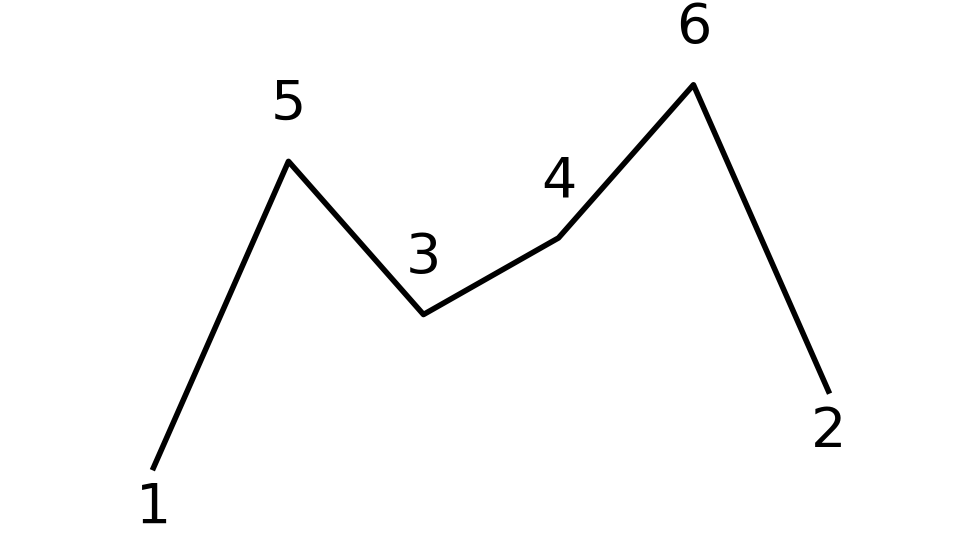
\includegraphics[width=3.5cm]{Introduction/op_P.png} & $T=$ \underline{2 7 4 5 8 3} \underline{1 20 15 16 25 6}  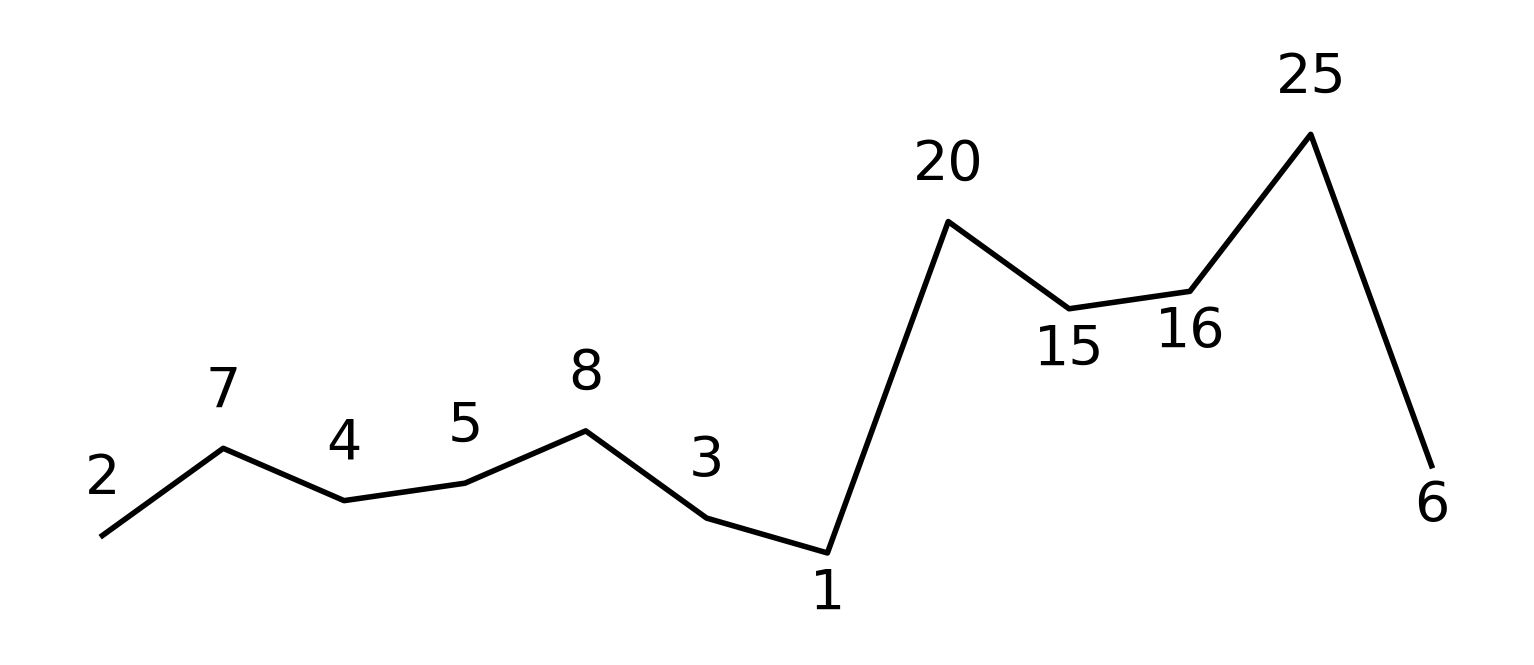
\includegraphics[width=5cm]{Introduction/op_T.png} \\
        %
        Parametrized~\cite{baker1993theory} & $P=$ GATTACAT & $T=$ OPO\underline{POGGODOG}O, {\footnotesize A:O, C:D, G:P, T:G} \\
    \end{tabularx}
    \caption{Example of various model of matching on strings.}
    \label{fig:intro:match_model}
\end{figure}

However, the need for text processing goes far beyond exact matching of patterns. To illustrate this claim, we present models of matching (underlined) relevant to this thesis with their motivations and specify those we study in the following chapter. Figure~\ref{fig:intro:match_model} also provides an example for each matching model.

% Regular expression
One of the oldest and most classic models for more complex queries is \ul{regular expressions} search, introduced by Kleene in 1951~\cite{RM-704}.
% Explain the formalism
The regular expression formalism offers a concise description for sets of strings through recursive combinations of characters from an alphabet $\Sigma$ along with three fundamental operators: concatenation ($\cdot$), union ($|$), and Kleene star ($\ast$).
For two regular expressions $R_1$ and $R_2$ the concatenation $R_1\cdot R_2$ matches any concatenation of a string matching $R_1$ and a string matching $R_2$, the union $(R_1|R_2)$ allows matching any string matching either $R_1$ or $R_2$, and $(R_1)^\ast$ matches any number of repetitions of a string matching $R_1$, including no repetition, i.e. the empty string.
% Application
The use of regular expression gained popularity in the 1970s through their efficient implementation in Unix tools such as awk, grep, or sed.
They have become a crucial tool in many fields such as internet traffic analysis~\cite{4221791,4579527}, databases, data mining~\cite{1000341,10.5555/645927.672035,10.1145/375551.375569}, computer networks~\cite{10.1145/1159913.1159952}, and protein search~\cite{10.1145/369133.369220}.
% automaton
Another way to describe regular expressions is through the Thompson automaton construction~\cite{Thompson_automaton}. This automaton can then be simulated efficiently to test whether a string $T$ is recognized by a regular expression $R$ in $\Oh(|R| \times |T|)$ time.
% Lowerbounds
A series of works~\cite{10.1145/128749.128755,BILLE2008486,10.1007/978-3-642-02927-1_16,10.1007/11786986_56,doi:10.1137/1.9781611973075.104} has focussed on improving the time complexity of regular expression search. However, they only managed to shave off polylogarithmic factors from the $\Oh(|R| \times |T|)$ complexity, and a recent fine-grained complexity approach brought an explanation for this.
Backurs and Indyk~\cite{DBLP:conf/focs/BackursI16} followed by Bringmann, Gr{\o}nlund, and Larsen~\cite{8104068} considered a subclass of regular expressions called ``homogeneous''. A regular expression is ``homogeneous'' if, in the tree representation of the expression, the operators at the same level are equal. For example $R=(P_1|P_2|...|P_d)^\ast$ is homogeneous and searching it corresponds to the Word break problem~\cite{wordbreak1,wordbreak2}. The authors of~\cite{DBLP:conf/focs/BackursI16,8104068} showed that every homogeneous regular expression search either allows for a solution in near-linear time or requires $\Omega((|R| \times |T|)^{1-\alpha})$ time conditioned on the Strong Exponential Time Hypothesis~\cite{IMPAGLIAZZO2001367}. The only exception is the Word break problem which can be solved in $\Oh(n (m \log m)^{1/3}+m)$-time has a matching lower bound up to polylogarithmic factors. Abboud and Bringmann~\cite{DBLP:conf/icalp/AbboudB18} further detailed those lower bounds using an even finer-grained complexity approach.
% Our work
These results give a good understanding of the time complexity of regular expression in the classical setting, however, multiple practical applications need to work with a stream of input. We specify what we mean by a stream later on in this introduction. Therefore, in Chapter~\ref{chap:regexp}, we provide a new space-efficient streaming algorithm for regular expression membership and pattern matching.


% Don't care
Although the versatility of regular expressions makes them widely used in practice across fields, they are notoriously difficult to write for users.
As a simpler alternative, Fischer and Paterson~\cite{fischer1974string} introduced the \underline{``don't care''} pattern matching where a don't care (also called wildcard or gap) symbol, denoted \texttt{?}, can occur in both the pattern and the text, and matches any other character of the alphabet.
% Space seed
This model has been directly applied in the PROSITE~\cite{hulo2006prosite} database of proteins where wildcards are supported. More generally, space seeds~\cite{li2004patternhunter}, a similar concept where only some positions have to be matched, have been used in homology search~\cite{ma2002patternhunter}, alignment~\cite{david2011shrimp2}, assembly~\cite{birol2015spaced}, and metagenomics~\cite{bvrinda2015spaced}.
% Gapped matching
Patterns with don't cares are sometimes~\cite{lewenstein2011indexing} described as $P= P_1g_1P_2g_2 \dots g_\ell P_{\ell+1}$ where $P_1$,$P_2$,\dots,$P_{\ell+1}$ are patterns over the alphabet $\Sigma$ and $g_1,g_2,\dots,g_{\ell}$ are the length of the maximal stretches of \texttt{?}. 
% variable length gap
Naturally this question was later extended to the problem of string matching with \underline{variable length gap}~\cite{bille2012string,bille2014string} where the length of the gaps can vary in intervals $[a_i,b_i]$ for $i\in[1,\ell]$.
% Applications
Note that variable length gaps are also supported by the PROSITE~\cite{hulo2006prosite} database.
% variants
Different variants of the problem have been studied~\cite{kopelowitz2016color,cohen2009range,brodal1999finding}, including a simpler version with just two patterns $P_1$ and $P_2$ and a single gap~\cite{peterlongo2006gapped,iliopoulos2009indexing} and the special case $P_1=P_2$~\cite{muthukrishnan2002efficient,keller2007range}.

% consecutive
In 2016, Navarro and Thankatchan~\cite{NAVARRO2016108} proposed a natural variant to pattern matching with a variable length gap, where given a single pattern $P$ and an interval $[a,b]$, one must report all consecutive occurrences of $P$ starting at positions $(i,j)$ (consecutive meaning no other occurrence in between $i$ and $j$) such that $j-i$ belongs to $[a,b]$. Since, consecutive occurrences have been studied in several publications~\cite{DBLP:conf/fsttcs/BilleGPRS20,cpm/BilleGPS21,DBLP:journals/corr/abs-2304-00887,DBLP:journals/corr/abs-2211-16860}.
% Gapped consecutive matching
Recently Bille et al.~\cite{bille2022gapped} proposed a combination of the gapped and consecutive lines of research: \underline{gapped consecutive matching} where we are given two patterns $P_1$ and $P_2$ as well as an interval $[a,b]$ and must report all consecutive occurrences of $P_1$ and $P_2$ with distance in $[a,b]$.
% Motivations
%This model can be linked to gapped q-grams~\cite{burkhardt2003better} which is an alternative to spaced seeds which were mentioned earlier.
% This thesis
We study gapped consecutive pattern matching in various settings in Chapters~\ref{chap:gapped_index} and~\ref{chap:gapped_pm}, a summary of the contribution is given in Section~\ref{intro:sec:contrib}.
%~\ref{chap:gapped_stream},

Although an in-depth non-standard matching listing is out of scope for this manuscript, for completeness, we detail other models found in the literature, and Table~\ref{fig:intro:match_model} provides exemples for each of the models.
% Degenerate strings
The modelling of flexible and diverse DNA sequences~\cite{comm1970iupac} lead to the model of \underline{degenerate} strings~\cite{abrahamson1987generalized} (also called indeterminate), where each position corresponds to a subset of $\Sigma$.
% (Elastic/Generalised) Degenerate strings
This model has recently been extended in two directions: \underline{elastic degenerate} strings~\cite{iliopoulos2021efficient} where each position is a subset of strings over $\Sigma$ and \underline{generalized degenerate} strings~\cite{alzamel_et_al:LIPIcs:2018:9323} where each position is a subset of strings of $\Sigma^k$, and the length $k$ can vary from position to position.
% Weighted string
Alternatively, when each position is assigned a random variable with values in $\Sigma$ the strings are called \underline{weighted} (or uncertain) and represented by a weight matrix~\cite{thompson1994clustal}, see Table~\ref{fig:intro:match_model} for an example. Then, the cumulative probability that a string occurs at a starting position is the product of the probabilities of the corresponding characters at each position, and a match is often defined by a threshold on that cumulative probability. This model has been used in molecular biology in ``profiles'' that represent multiple aligned strings~\cite{doi:10.1073/pnas.84.13.4355} though they study a slightly different score: $\log \frac{p(x,i)}{p(x)}$ where $p(x,i)$ is the probability that the $i$th character is equal to $x$ and $p(x)$ is the overall frequency of $x$. 
% Abelian/jumbled/many other names 
In the model of \underline{abelian} matching, a string (or a substring) is entirely identified by the characters it contains (with multiplicities), disregarding their order. It stems from the automatic discovery of clusters of genes in genomes where they can occur in a different order but still linked to the same function~\cite{eres2004permutation}, but the same concept has also been used in the context  of using mass spectrometry for DNA assembly~\cite{bocker2003sequencing} where the strings without order are called compomers. This model is also known as jumbled and permutation pattern matching, and several other names, see~\cite{ejaz2010abelian}.
% order preserving
The \underline{order-preserving} model~\cite{kim2014order,kubica2013linear} takes a somewhat opposite approach and says that two strings match if they have the same relative shape: $\forall i,j \in [0,n-1], X[i] < X[j] \leftrightarrow Y[i] < Y[j]$. This matching model aims at capturing the trend detection needed in the stock market and music melody matching problems~\cite{kim2014order}.
%
% Parametrized matching
Another application-driven model is \underline{parametrized strings} or ``p-string'' introduced by Baker~\cite{baker1993theory}, where two strings match if we can transform one into the other by applying a function renaming the parameters, meant to detect code duplication.

\subsection{Periodicity Detection}
\todo[inline]{Work in progress do not review!\\ TODO: Detail}
So far we focussed on matching models where we are given a pattern and text as well as conditions that define a match of the pattern in the text. But another central task in text processing is repetitions detection. By repetitions, we refer to consecutive occurrences of the same fragment. They can be repeated twice (a square), three times (a cube) or more, then represented as a run: a maximal periodic substring. They are needed as a theoretical tool to avoid needless repetitive computations, but they also naturally occur in DNA with an important role in genomic fingerprinting~\cite{Kolpakov2003}.
The study of squares in strings goes back to 1906 with the work of Thue~\cite{thue1906} on the construction of an infinite square free string, in Chapter~\ref{chap:squares} we provide an optimal algorithm for square detection.

% Should also define runs
% Mention palindromes and stuffs ?

\subsection{Similarity Measures and Distances}
\todo[inline]{Work in progress !}
% The notion of robustness of the similarity measure
% Similarity measures
Many string applications have to work around noise in the input data, which makes it difficult to search for exact matches. Some of the models presented earlier define their match to take into account noisy input, but another important approach is to work with distances and similarity measures. Quantifying the degree of similarity and dissimilarity of two strings is for example needed in Bioinformatics~\cite{Gusfield1997}, music analysis~\cite{mongeau1990comparison} and plagiarism detection~\cite{lukashenko2007computer}. 
%
A distance measure quantifies the dissimilarity between strings, while a similarity measure quantifies the degree of resemblance between strings. Most distances can be derived into similarity measure, and most similarity measure have a corresponding distance, thus in this section we alternate between the two terms depending on which form is most common in the literature.

% Robustness to noise
There are various type of noise that can appear in the input, examples include single characters or entire words being replaced, inserted, or deleted, some sections of the text being stretched or reordered. Consequently, there are various similarity measure that can account for the different types of noise, as the goal is always that a few noisy modifications does not modify drastically the distance to other strings.
% Hamming
One of the simplest distance on string is the \underline{Hamming distance}: For two strings $X$ and $Y$ with $|X|=|Y|$ it is the number of mismatches between $X$ and $Y$. Alternatively, the Hamming distance is defined as the number of substitutions needed to transform $X$ into $Y$.
% Longuest Common Subsequence
When instead the goal is to have a similarity measure robust to insertions and deletions in the strings $X$ and $Y$, one can consider the length of the \underline{Longest Common Subsequence} between $X$ and $Y$. That is finding the largest $\ell$ such that there exist positions $i_1<... < i_\ell$ and $j_1< ... < j_\ell$ such that $X[i_p] = Y[j_p]$ for all $p \in [1,\ell]$. Note that the longest common subsequence has been used as the basis of comparison program like \texttt{diff} which are then applied in version control system like git.
% ED / Levenshtein
For the \underline{Levenshtein distance}~\cite{levenshtein1966binary} (also called edit distance) the operations allowed are substitutions, insertions and deletions. This metric is one of the most well known, due to the importance of finding global alignments (alignments of the two string with substitutions, insertions and deletions) in bioinformatics~\cite{Gusfield1997}.
%\todo[inline]{Add the Jarno-Winkler distance which allows translocations ?}
Unfortunately, Backurs and Indyk~\cite{DBLP:conf/stoc/BackursI15} proved a conditional lower bound (based on SETH) which suggests it is unlikely to be computable in strongly subquadratic time.
% LCS with $k$ mismatches
Therefore, in Chapter~\ref*{chap:LCS} we consider another similarity measure resilient to substitutions: \kApproxLCS which is an approximate version of \kLCS . In the \kLCS problem, given an integer $k$ and two strings $X$ and $Y$, $\lcsk(X,Y)$ we must compute the maximal length of a substring (not subsequence) of $X$ that occurs in $Y$ with at most $k$ mismatches. 
But again, Kociumaka, Radoszewski, and Starikovskaya~\cite{DBLP:journals/algorithmica/KociumakaRS19} showed (conditioned on SETH) that there is $k=\Theta(\log n)$ such that \kLCS cannot be solved in strongly subquadratic time, thus they introduced \kApproxLCS . In that problem we are given a constant $\eps > 0$, and need to return a substring of $X$ of length at least $\lcsk(X,Y)$ that occurs in $Y$ with at most $(1+\eps) \cdot k$ mismatches.
In Section~\ref{intro:sec:contrib}, we explain our contributions to the study of that similarity measure.

% Approximate matching
Apart from the direct comparison of two strings, distances are also used to define approximate matching problems~\cite{landau1986efficient,landau1989fast} where for given an integer $\tau$, a pattern $P$ and a text $T$, one must report all positions $j$ such that there is a substring $T[i..j]$ that is at distance at most $\tau$ from $P$.
% DTW
We study approximate matching in Chapter~\ref{chap:DTW} according to a popular distance for temporal sequences but less common for strings: the \underline{Dynamic Time Warping (DTW) distance}~\cite{sakoe1978dynamic}. For strings, the DTW distance can be described as follows: double some characters to obtain strings of equal length and in order to minimize the sum of the distances between the characters at the same positions, this sum is the DTW distance.
%
All similarity measures and distances mentioned above are illustrated in Figure TODO.
\todo[inline]{Have a figure illustrating of each similarity measure/distance.}
% PM


%also need relevant and efficient similarity measures such as the Levenshtein distance or Dynamic Time warping distance~. They also often need to report all occurrences with an error bound\: at a distance at most a threshold $\tau$.
%We contribute to this line of research in Chapters~\ref{chap:LCS} and~\ref{chap:DTW}.


\subsection{Scalability Issues}\label{sec:intro:scalability}

%%%%%%%%%%%%%%%%%%%%%% Intro scalibility %%%%%%%%%%%%%%%%%%%%%%%%%%%%
 
% But it is not just about the specific model also about scalibility
We discussed so far how string processing tasks have crucial industry-relevant applications, but another major challenge in most applications is the scalability to large datasets.
% Wikipedia
Highly curated datasets generally remain quite small, for example the English pages of Wikipedia (just the text and metadata) take up 20~gigabytes in a compressed format as of 2022~\cite{wikimedia}. In comparison, any form of archival and version history tends to grow much bigger. Just the metadata of revision's history (without the content of the articles) for the Wikipedia English pages takes up 75~gigabytes as of 2022.
% Software Heritage
It is sometimes possible to limit the redundancy in the archival data, for example by using a graph which tracks where the data is repeated multiple times. This is the approach taken by the Software Heritage~\cite{swh-site} project, which aims at keeping an archive of entirety of the software code produced by humanity. The graph structure is especially necessary in this project to reduce code redundancy and reflect the standard use of version history management in software development.
Substantial research and engineering effort~\cite{DBLP:phd/hal/Pietri21} were made to provide an efficient navigation of the graph. 
However, since the code repositories are indexed based on their URLs and metadata, it is not currently feasible to perform a search specifically for occurrences of a particular code snippet\footnote{\setlength\parindent{10pt} A silly but interesting example is~\cite{vii2014if} where the author searched \texttt{"const double epsilon ="} (and equivalents in other languages) on all GitHub repositories to study the value programmers typically chose for epsilon.}.
As of 2023, the graph is limited to 7~terabytes but with the source files the space usage approaches 1~petabyte~\cite{swh-polytechnique}.
% Internet archive
Another example of a large archival project is the internet archive, a non-profit which started saving web pages in 1996 and now holds the history of more than 800 billion web pages through their program: the wayback machine~\cite{web-archive}. This archive takes up more than 70~petabytes, however, one of the limitations is that the search options are limited to the metadata of the websites and not the content of the webpages themselves.


%%%%%%%%%% Bioinformatics
%Intro DNA representation
Large archives also exist in bioinformatics, but the structure of biological sequences is very different from that of code or webpages.
DNA is typically stored as a string over the nucleotide alphabet \texttt{\{A,T,C,G\}} which can be stored using just 2 bits per base. However, this type of storage requires scanning the whole string to search for a pattern. 
At the opposite of the spectrum, a suffix tree enables more efficient sequence analysis but necessitates 10 bytes per base~\cite{navarro2016compact}, which amounting to 30 gigabytes for a human genome containing 3.3 billion bases. 
And thousands of genomes have been sequences through projects such as the 1000 Genomes project~\cite{10002015global} completed in 2015 and the 100K Genomes project~\cite{100Kgenomes} which reached its milestone in 2018. 
A trade-off between those two extremes has been found through the development of compact data structures that exploit redundancy to decrease space usage. For a human genome it allows representing the sequence and its suffix tree using just 4 gigabytes~\cite{navarro2016compact}.
% Redundancy intra genome and intergenome
The redundancy that compact data structures can exploit in genomes can come either from repeated regions in the genome (intra-genome redundancy) or by considering several genomes (from the same specie) that share portions of their genomes (inter-genome redundancy).  
% Reads
However, for DNA, another common data model is the one of reads: when DNA is sequenced, the output is a set of fragments (called \emph{reads}) of the original sequence. Reads can contain sequencing errors, including nucleotide insertions, deletions, and substitutions. The typical length and error rate of the reads vary depending on the sequencing techniques. To be able to reconstruct the original sequence, reads are extracted in such quantities that each position of the original genome is covered multiple times. This means readsets are larger than the assembled genome and even more redundant. In Chapter~\ref{chap:XBWT} we explore this topic for short reads and propose a data structure specifically tailored to the specificities of a sequencing technique. 
% Cheaper = more sequencing
Additionally, the drastic decrease in sequencing cost and increase in throughput since 2008 (faster than expected by Moore's law~\cite{muir2016real}) have lead to higher volumes of DNA being sequenced. 
% ENA
So far, the European Nucleotide Archive has accumulated more than 47 petabytes~\cite{ena} of sequencing data.
% SRA
While the NCBI Sequence Read Archive has more than 73 petabases~\cite{sra} of archive including 38 petabases in open access. However, like for the software heritage project and internet archive, in the ENA and the NCBI, the data is indexed solely based on its metadata.\\
%\todo[inline]{Look for more reasonable size example ? It's unclear if anybody would want to index the entire SRA}

%%%% Astronomical data 
\todo[inline]{Add applications to astronomical data and pulsar detection.}
%\todo[inline]{Add one or several graphs illustrating the growth in data in each field.}

\begin{figure}
    \centering
    \begin{subfigure}[b]{0.45\textwidth}
        \begin{tikzpicture}
            \node (img) {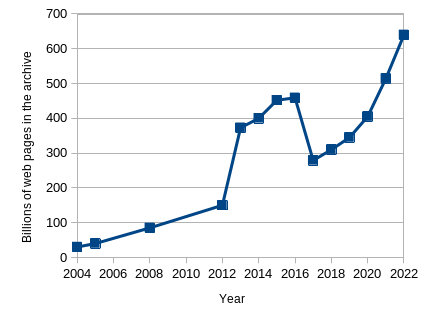
\includegraphics[width=\textwidth]{0_sheets/wayback_machine.png}};
            \node [below right,text width=2.7cm,align=center, fill=white] at (0.25,-0.5){{\fontsize{7pt}{6pt}\selectfont Pages removed due to security concerns.}};
            \draw[->] (1,-0.5) -- (1.3,0.3);
        \end{tikzpicture}
        \caption{The Wayback Machine Archive}
    \end{subfigure}
    \begin{subfigure}[b]{0.49\textwidth}
    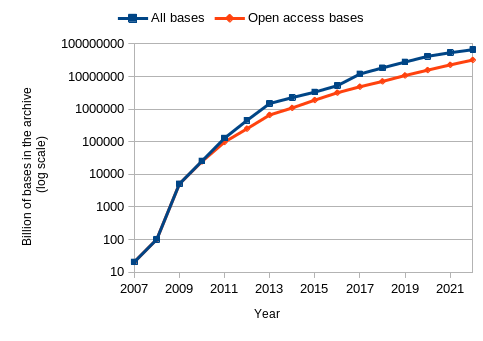
\includegraphics[width=\textwidth]{0_sheets/sra_growth.png}
    \caption{The Sequence Read Archive}
    \end{subfigure}
    \caption{Plots of the database growth for the Wayback Machine~\cite{web-archive-growth} and the Sequence Read Archive~\cite{sra}. The databases are big but also still quickly growing.}
\end{figure}

%%%%%%%%%%%%%%%%%%%%%% Approaches to adress scalibility %%%%%%%%%%%%%%%%%%%%%%%%%%%%
%
It goes without saying that algorithms with quadratic time complexity cannot scale to terabytes and petabytes of inputs. Consequently, the choice of matching model is dictated both by the specific needs of the application and the typical scale of the input.
%
Also note that some applications require \emph{data structures}, which are algorithms where the complexity analysis is split in two parts: the \emph{construction} and the \emph{query}. The construction is generally more expensive and meant to be performed once, whereas the queries are meant to be fast and performed multiple times with varying input-query. For example, Chapters~\ref{chap:gapped_index} and~\ref{chap:XBWT} build data structures.

Several approaches can be used to cope with large amounts of data, such as distributed algorithms that are designed to work on several computers sharing a network (with limited transfer). In this thesis, we focus on a different approach to process massive string data, that of sketching. A \textbf{sketch} is a lossless or lossy compression that keeps only the essential characteristic of the input needed to answer a given query, offering promising scalability potential. Example of sketches include Karp--Rabin fingerprints for lossy compression (see Preliminaries~\ref{sec:prelim:KR}) and Lempel--Ziv factorization for lossless compression (see Preliminaries~\ref{sec:prelim:compress}). 
We will detail in Section~\ref{intro:sec:contrib} how each contribution of this thesis relates to sketching but let us first summarize three general sketch-based approaches (that can sometimes be combined):
%summarize their respective scalability approaches as follows (with some approaches that can be combined): 

\begin{itemize}
\item Compressed input: as mentioned already, highly redundant data can sometimes be represented by a sketch of a more manageable size. 
Consequently, algorithms that can directly operate on the sketch become much more efficient. This is very natural approach as the data is almost always shared in a compressed format, the difficulty focusses on working with the sketch's property and structure. However, it is important to note that not all problems can be solved faster with this approach. For example, Abboud et al.~\cite{abboud2017fine} showed that to compute the longest common subsequence of two strings of uncompressed size $N$, given in a sketch of size $n$, there is a lower bound $(nN)^{1-o(1)}$ assuming the Strong Exponential Time Hypothesis (SETH). 
Very recently, Ganesh et al.~\cite{ganesh2022compression} also showed a lower bound $\Omega(N^{k-1}n)$ conditioned on SETH to compute the median edit distance and length of the longest common subsequence of $k$ strings.
In other words, even if the input is given compressed form, we cannot avoid a high dependency in the uncompressed size. In this thesis, Chapters~\ref{chap:gapped_pm} and~\ref{chap:gapped_index} both take as input a sketch, more precisely a grammar compressed text and their complexities are given as a function of the size of the compressed input.
\item Streaming algorithms: there, the data is considered so large that it can only be handled as a stream. % then it must be processed on the fly without the possibility of going back.
For the pattern matching problem, the pattern and the length of the text are known in advance and can be preprocessed, then the characters arrive one by one and can only be accessed later if they are stored explicitly. 
This model focusses on small space complexity and accounts for every extra space needed apart from the current character. Thus, sketches are crucial to keep the necessary information about the data already seen while limiting space usage.
%This model optimizes both the time per character during the streaming phase and the space complexity which accounts for storing the result of the preprocessing and any space necessary to process the characters.
Chapter~\ref{chap:regexp} is set in this model. %~\ref{chap:gapped_stream}
%
Those streaming algorithms relate in practice to the notion of efficient second-memory algorithms. One of the challenges when dealing with large inputs is the quantity of main memory used, as most computers are still limited to gigabytes of RAM. To circumvent this limitation, programs may resort to working directly from secondary memory as disk space scales at a much cheaper cost than RAM.
It is  common knowledge that random access to disk is very inefficient, however contiguous reads on recent SSD can read gigabytes (between 2.2 and 3.4 Gb) of data per second which is comparable to the speed of most RAM. %which is either comparable to the speed of reading from main memory or only 10 times slower (depending on the model of RAM).
Therefore, an algorithm that uses few random accesses (including streaming algorithms) can be executed directly on disk which allows it to scale to large inputs much more easily. 
%The main issue with this approach is that not all problems admit efficient solutions avoiding random access. For example, given a list and a permutation, returning the permuted list requires to access the elements in the order of the permutation, possibly random. 
We use this approach of streaming on secondary memory to limit main memory usage in Chapter~\ref{chap:XBWT}. The construction of the index is split in phases that read contiguously from disk, process the information (for the next phase or final output) and write to disk.
\item Approximation algorithms: When dealing with very large datasets, it is not always needed to provide precise answers to queries. Allowing for some approximation in the results can enable shortcuts and help bypass lower bounds. There, using sketches in the form lossy compression inherently introduces approximation but allows for even smaller and more efficient representations.
The entire second part of this thesis is dedicated to this approach, and Chapter~\ref{chap:LCS} stands out as a particularly representative example. We treat the problem of the Longest Common Subsequence with approximately $k$ mismatches with a probabilistic algorithm that answer correctly with high probability. %($\geq 1 - \frac{1}{n}$ for an input of size $n$).
\end{itemize}

